\chapter{Experiments}

\section{Classical Computer Vision-based Approach}

\subsection{Gaze Projection}
\begin{figure}
    \centering
    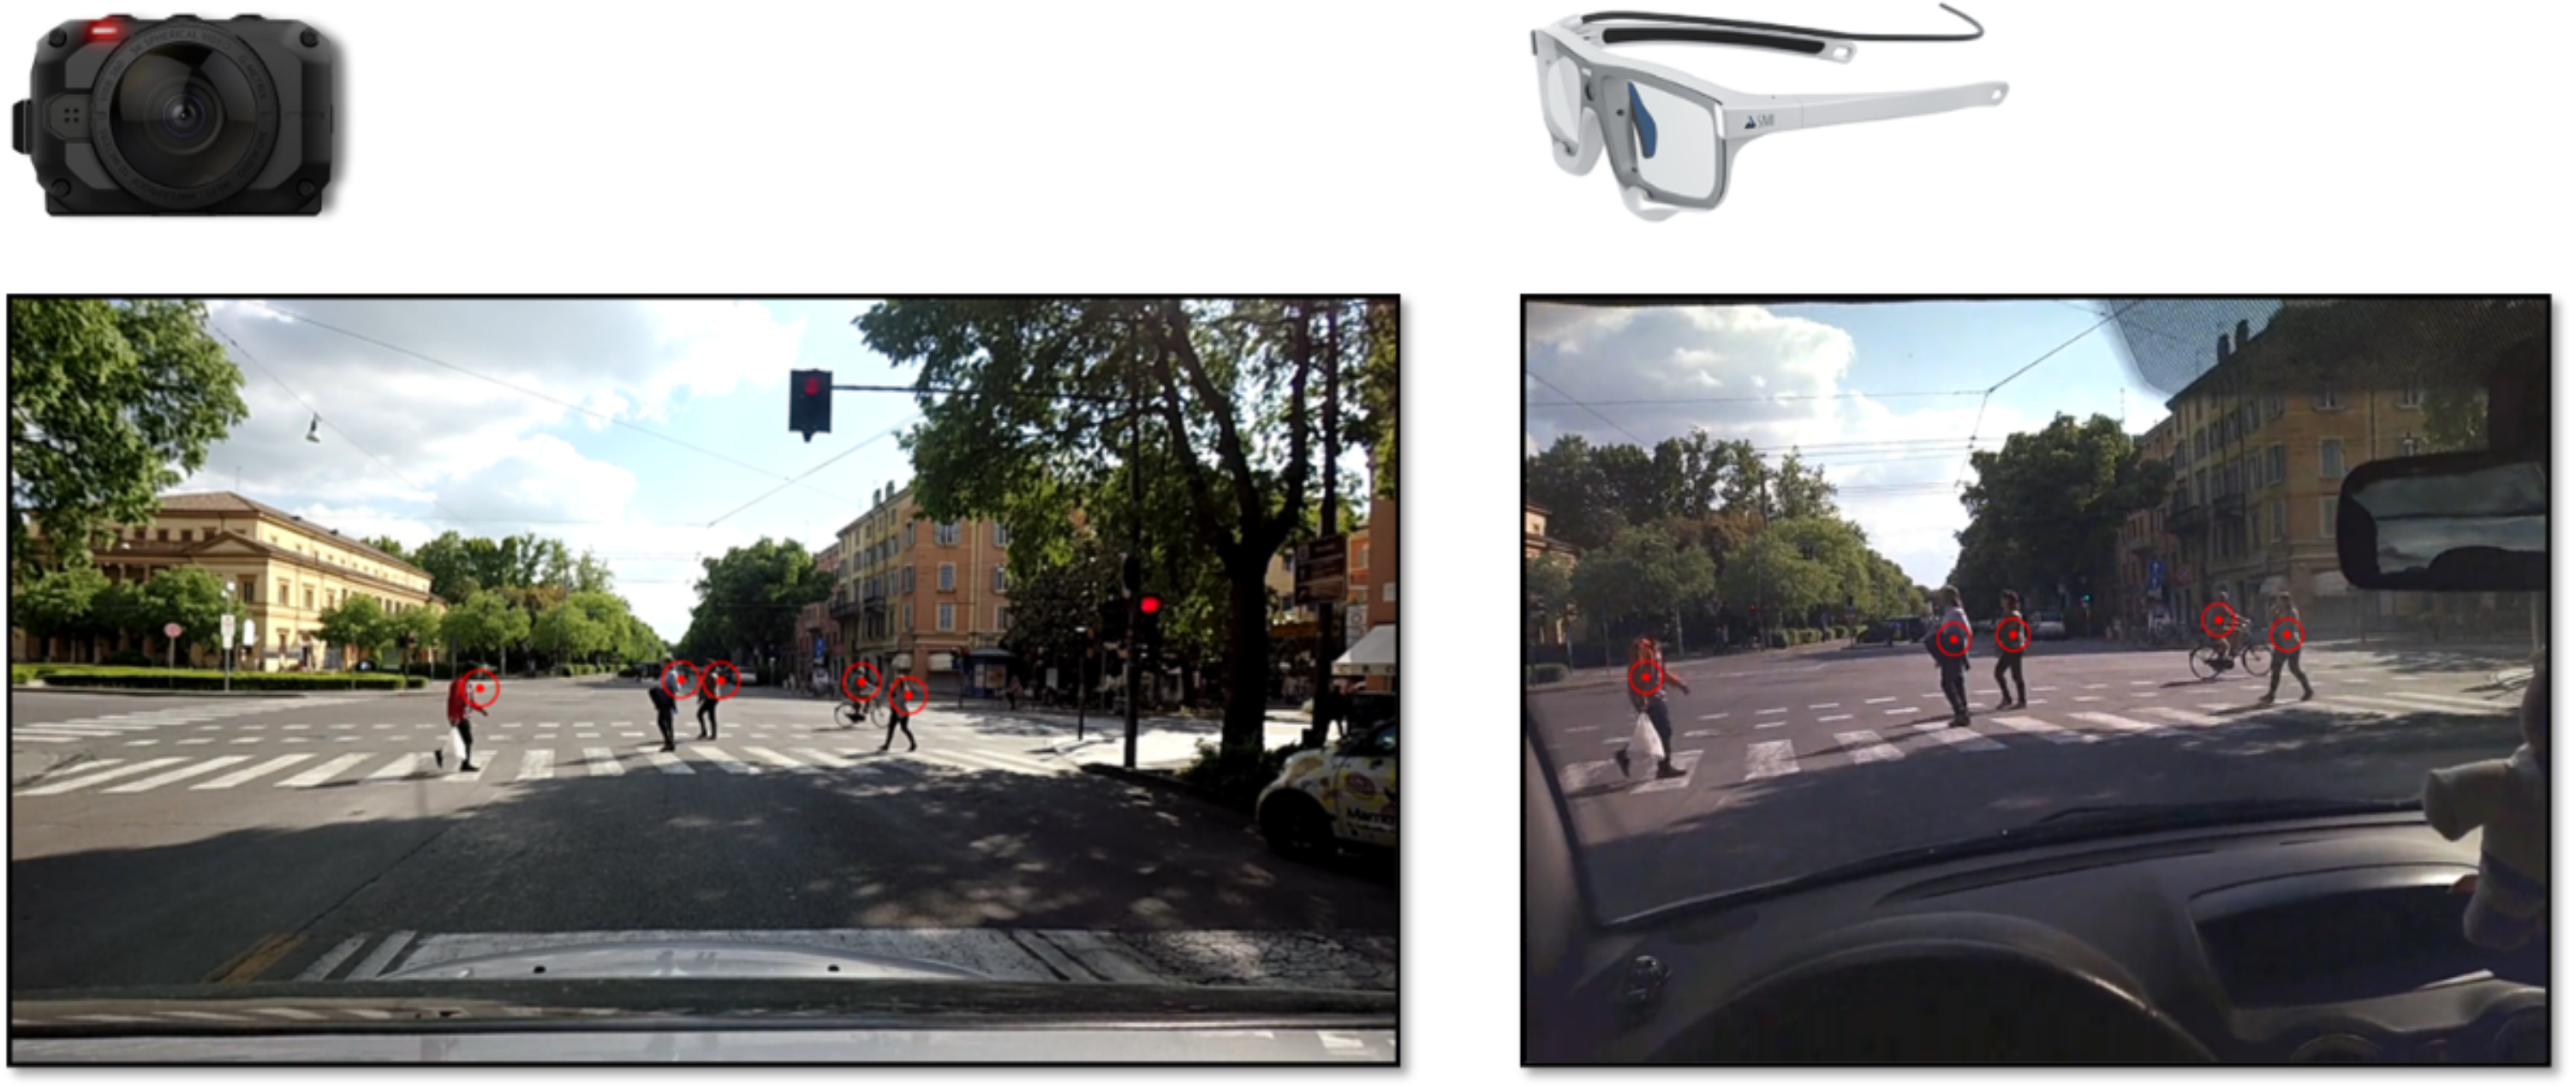
\includegraphics[width=\textwidth]{images/dreyeve/gaze_projection.png}
    \caption{Projection of the gaze from the ETG camera to the RT camera. 
    All the gaze points are manually set.
    \textbf{Left}: Roof top camera view.
    \textbf{Right}: ETG camera view.}
    \label{fig:gaze_projection}
\end{figure}
\begin{figure}
    \centering
    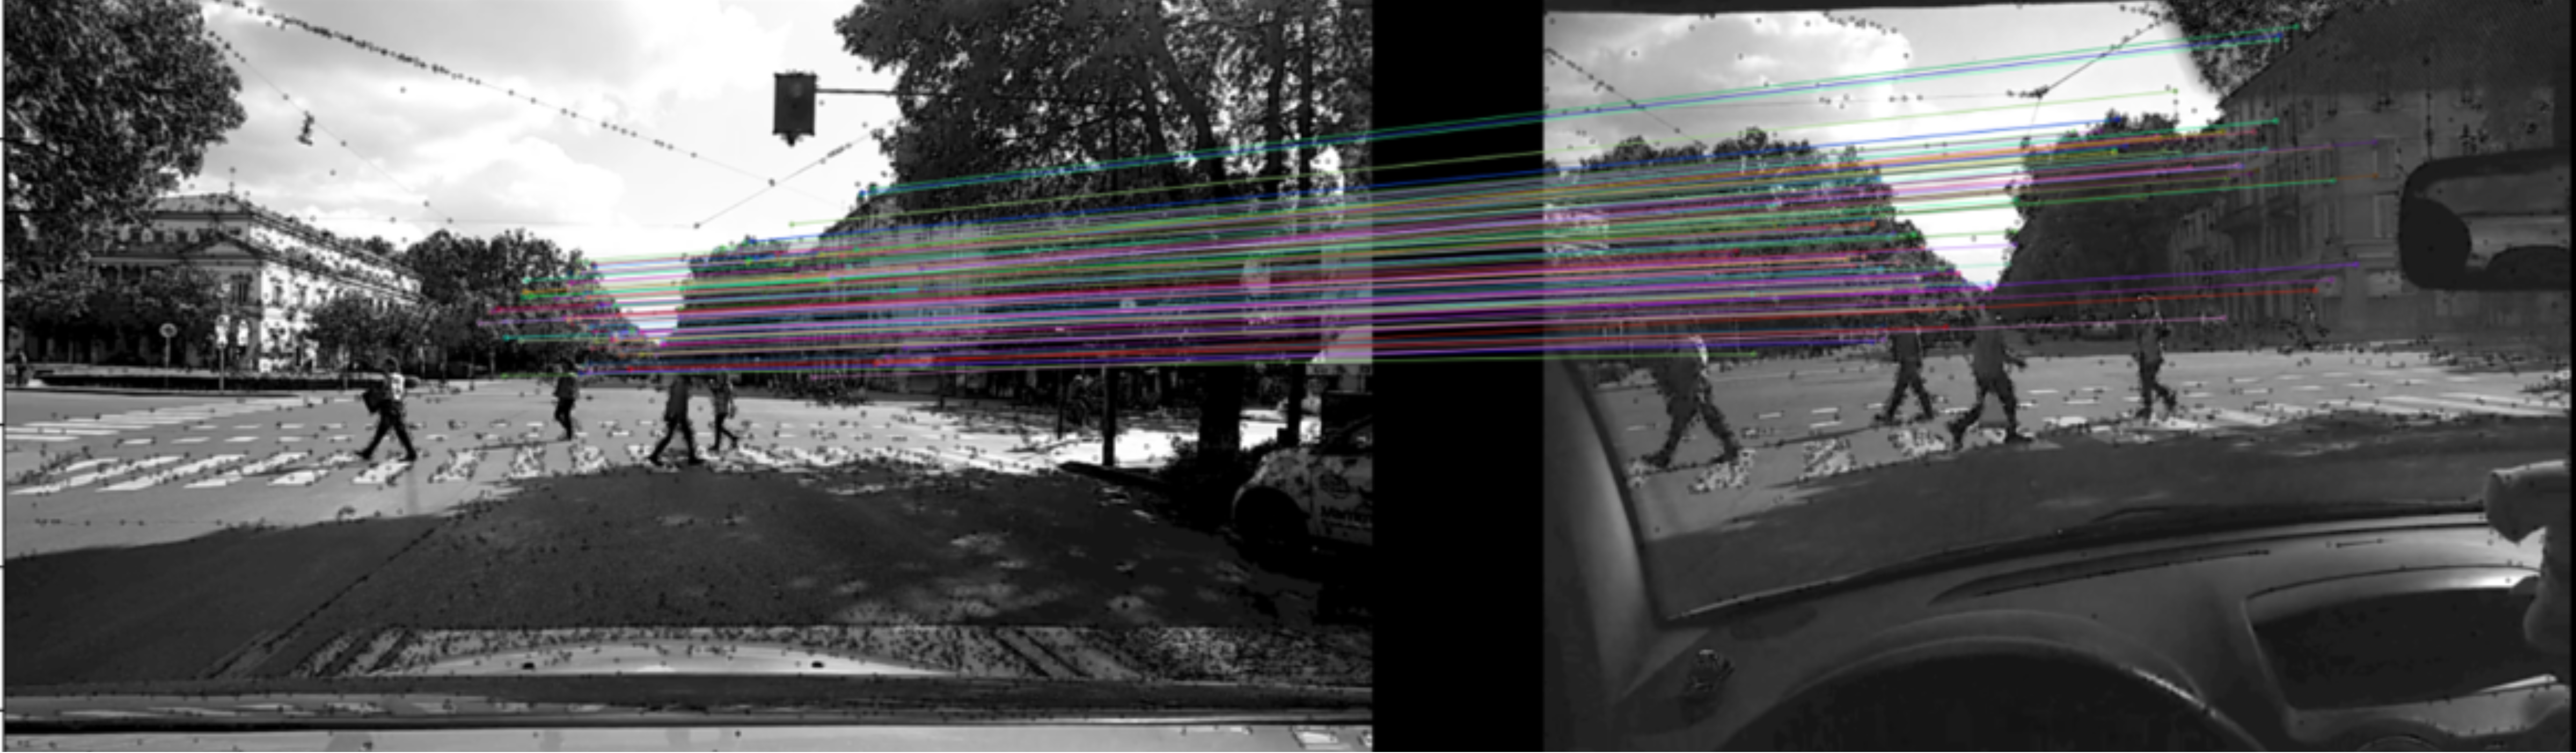
\includegraphics[width=\textwidth]{images/dreyeve/gaze_matchings.png}
    \caption{Projection of the gaze from the ETG camera to the RT camera. 
    All the gaze points are manually set.
    \textbf{Left}: Roof top camera view.
    \textbf{Right}: ETG camera view.}
    \label{fig:gaze_matchings}
\end{figure}
The projection of the gaze from the ETG camera to the RT camera is shown in 
Figure \ref{fig:gaze_projection}. We manually set some gaze points on the 
ETG camera such that they overlap with the vulnerable users. In this way, 
we are setting some operation points that we can use to evaluate the quality 
of the homography estimation. From the figure it is possible to see that the 
projection is not perfect, but it is a good approximation of the gaze in the 
RT camera plane. The small errors are due to the fact that the scene is not 
flat and the homography is a planar transformation. However, most pixels with 
high contrast correspond to objects that are far away from the vehicle, 
therefore the approximation is reasonable.

\subsection{Distribution of People in Dr(eye)ve}
\subsection{Gaze Interaction with Targets}
\subsection{Adding Depth Information}
\subsection{Adding Spatial Information}


\section {Deep Learning-based Approach}
\subsection{Supervised Training on Dr(eye)ve}
\subsection{Semi-Supervised Training on Dr(eye)ve}
\subsection{Supervised Training on BDD100k}
\subsection{Semi-Supervised Training on BDD100k}
\subsection{Experiments with GPT4-o}